\documentclass{standalone}
\usepackage{tikz}
\usepackage{ctex,siunitx}
\usepackage{tkz-euclide}
\usepackage{amsmath}
\usetikzlibrary{patterns, calc}
\usetikzlibrary {decorations.pathmorphing, decorations.pathreplacing, decorations.shapes,}
\begin{document}
\small
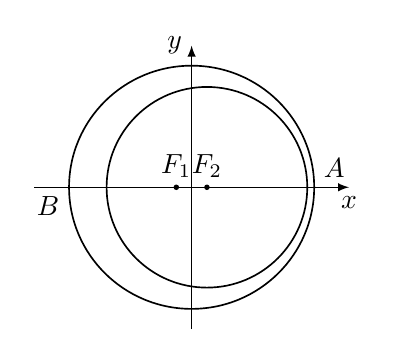
\begin{tikzpicture}[>=latex,scale=0.2]
  \draw[thin,->](-10,0)--(10,0)node[below]{$x$};
  \draw[thin,->](0,-9)--(0,9)node[left]{$y$};
  \draw[semithick](0.9725,0)circle(6.371);
  \draw[semithick](0,0)ellipse(7.783 and 7.722);
  \fill(-0.9725,0)circle(5pt)node[above]{$F_1$};
  \fill(0.9725,0)circle(5pt)node[above]{$F_2$};
  \node at (7.783,0)[above right]{$A$};
  \node at (-7.783,0)[below left]{$B$};
\end{tikzpicture}
\end{document}